\begin{align}
    \Vec{B-A} &=\myvec{
    2\\3
    } -\myvec{
    -1\\2}
\\ \label{3/4/5/eq1}
&= \myvec{3\\1}
\\ \Vec{C-A} &=\myvec{
4\\-3
} -\myvec{
-1\\2 }
\\
\label{3/4/5/eq2}
&= \myvec{5\\-5}
\end{align}
The area of the triangle is given by 
\begin{align} \label{3/4/5/eq3}
\frac{1}{2}\norm {(\Vec{B-A})\times ( \Vec{C-A}) }
 \label{3/4/5/eq4}
%     \Vec{P}\times  \Vec{Q}  = 
%     \myvec{
%     0&-a_{3}&a_{2}\\
%     a_{3}&0&-a_{1}\\
%     -a_{2}&a_{1}&0\\
%     }
%     \times \myvec{
%     b_{1}\\
%     b_{2}\\
%     b_{3}\\}
% \end{align}
% Substituting values from equation \eqref{3/4/5/eq1} and \eqref{3/4/5/eq2} in above equation \eqref{3/4/5/eq4}, we'll get:

% \begin{align}
%     \Vec{(B-A)}\times  \Vec{(C-A)}  = 
\\ &=    \myvec{
    0&0&1\\
    0&0&-3\\
   -1&3&0\\}
    \times \myvec{
    5\\
    -5\\
    0\\}
% \end{align}
% \begin{align} \label{3/4/5/eq5}
   % \Vec{(B-A)}\times  \Vec{(C-A)}   
    &= \myvec{0\\
   0\\
    -20\\}
% \end{align}
% \begin{align} \label{3/4/5/eq5}
\implies \norm {\Vec{(B-A)}\times  \Vec{(C-A)} } & = 20
\end{align}
which is the desired area.
%Substituting value from equation \eqref{3/4/5/eq5} in equation \eqref{3/4/5/eq3}, we'll get area of triangle:

% $
% \implies  \frac{1}{2}(20) =10 units^2
% $
\begin{figure}[h]
%\renewcommand{\theenumi}{1}
\centering
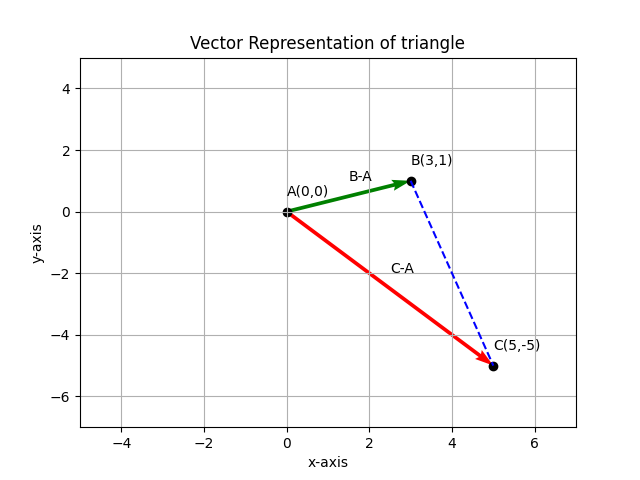
\includegraphics[width=\columnwidth]{solutions/3/4/5/image(graph).png}
\caption{Plot obtained from Python code}
\label{3/4/5/Fig:1}
\end{figure}
\end{document}
